\documentclass{exam}

\usepackage[utf8]{inputenc}

\usepackage{graphicx}
\usepackage{subcaption}
\usepackage{hyperref}
\usepackage{parskip}

\begin{document}

\title{
RE355: Cloud Computing - Docker
}

\author{Mathias Lacaud \\ Simon Da Silva}

\date{Monday October 23, 2017}

\maketitle

\begin{figure}[!htb]
	\centering
	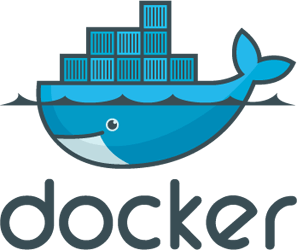
\includegraphics[width=.25\linewidth]{docker.png}
\end{figure}

\section{Introduction}

As you may not be comfortable yet with Docker, we provide you with a brief introduction before beginning the lab session. For more information, you can also browse the docker official website\footnote{\url{https://www.docker.com/what-docker}}.


\subsection{What is Docker?}

Docker is the world’s leading software container platform.

Developers use Docker to eliminate “works on my machine” problems when collaborating on code with co-workers.
Operators use Docker to run and manage apps side-by-side in isolated containers to get better compute density.
Enterprises use Docker to build agile software delivery pipelines to ship new features faster, more securely and with confidence for both Linux, Windows Server, and Linux-on-mainframe apps. 

\subsection{Why using Docker?}

Docker automates the repetitive tasks of setting up and configuring development environments so that developers can focus on what matters: building great software.
Developers using Docker don’t have to install and configure complex databases nor worry about switching between incompatible language toolchain versions.
When an app is dockerized, that complexity is pushed into containers that are easily built, shared and run.
Onboarding a co-worker to a new codebase no longer means hours spent installing software and explaining setup procedures.
Code that ships with Dockerfiles is simpler to work on: dependencies are pulled as neatly packaged Docker images and anyone with Docker and an editor installed can build and debug the app in minutes.

\subsection{What is a container?}

Containers are a way to package software in a format that can run isolated on a shared operating system.

Virtual machines run guest operating systems.
This is resource intensive, and the resulting disk image and application state is an entanglement of OS settings, system-installed dependencies, OS security patches, and other easy-to-lose, hard-to-replicate ephemera.

\begin{figure}[!htb]
	\centering
	\begin{subfigure}[!htb]{0.495\textwidth}
		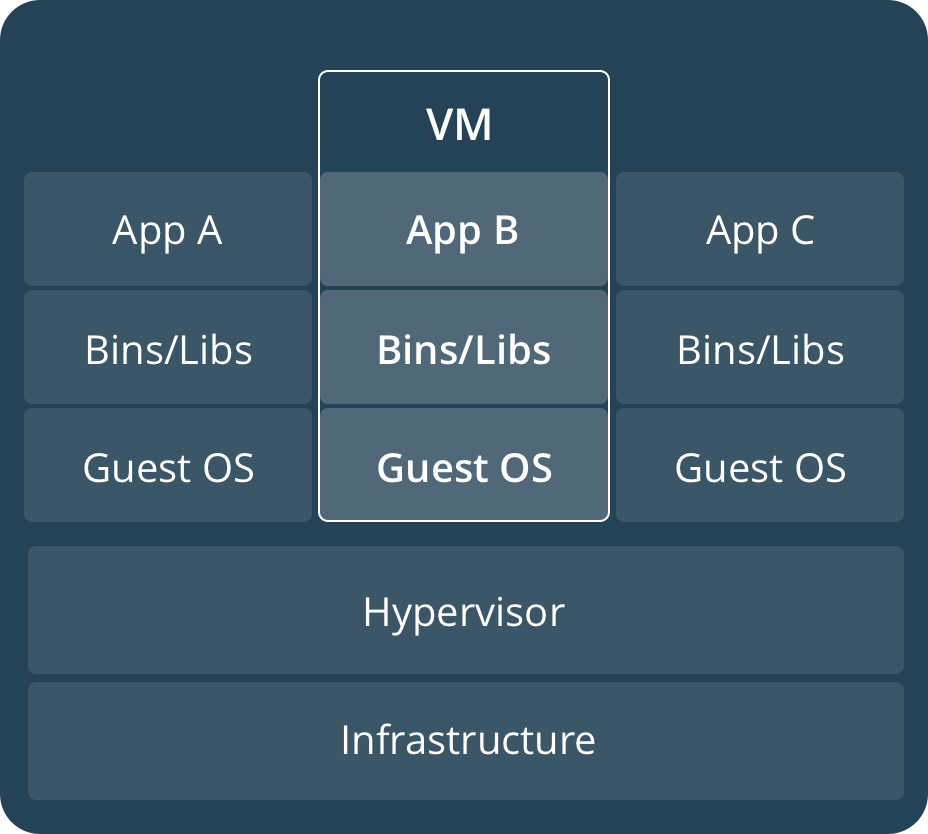
\includegraphics[width=\linewidth]{VM.png}
        \caption{Traditional Virtual Machine}
        \label{fig:VM}
    \end{subfigure}
    \hfill
	\begin{subfigure}[!htb]{0.495\textwidth}
		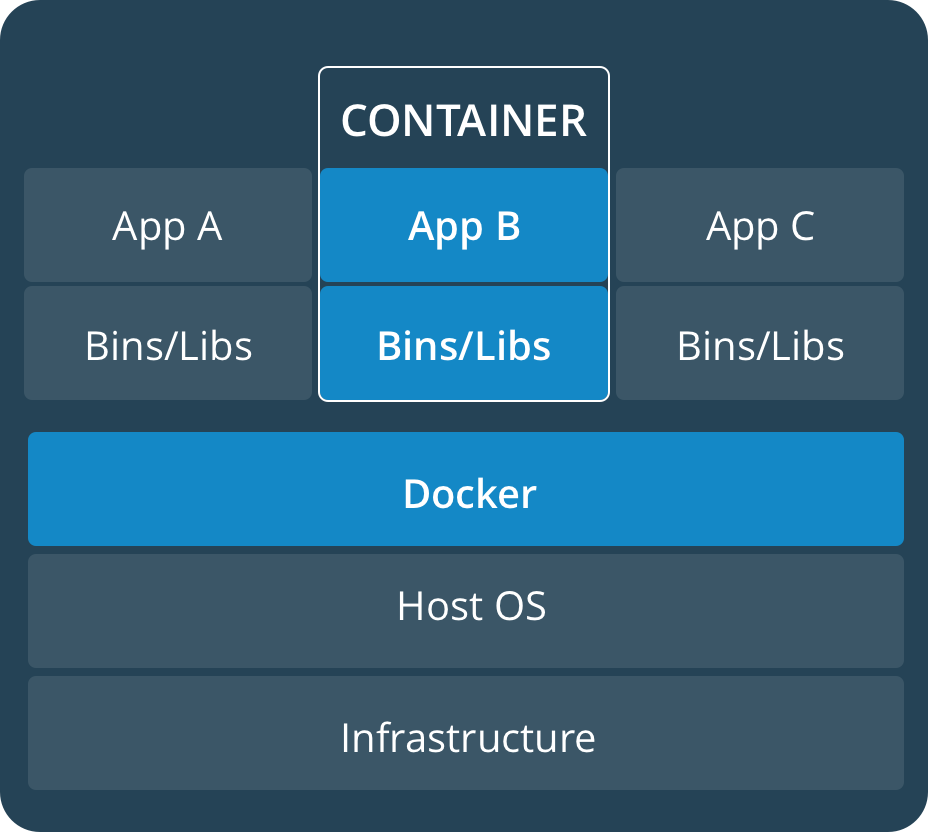
\includegraphics[width=\linewidth]{Container.png}
        \caption{Docker Container}
        \label{fig:Container}
    \end{subfigure}
	\caption{Comparison between visualization stacks 
    \label{fig:VMvsContainer}}
\end{figure}

Unlike VMs, containers do not bundle a full operating system.
Containers can share a single kernel, and the only information that needs to be in a container image is the executable and its package dependencies, which never need to be installed on the host system.
These processes run like native processes, and you can manage them individually.
Finally, because they contain all their dependencies, there is no configuration entanglement; a containerized app runs anywhere.
This makes for efficient, lightweight, self-contained systems and guarantees that software will always run the same, regardless of where it’s deployed.

\subsection{Docker terminology}

An \textbf{image} is a lightweight, stand-alone, executable package that includes everything needed to run a piece of software, including the code, a runtime, libraries, environment variables, and config files.

A \textbf{Dockerfile} defines what goes on in the environment inside your \textbf{container}.
The \textbf{Dockerfile} is then built into an \textbf{image}.
Access to resources like networking interfaces and disk drives is virtualized inside this environment, which is isolated from the rest of your system, so you have to map ports to the outside world, and be specific about what files you want to copy in to that environment.
However, after doing that, you can expect that the build of your app defined in this Dockerfile will behave exactly the same wherever it runs.

A \textbf{container} is a runtime instance of an \textbf{image}: what the image becomes when actually executed.
It runs completely isolated from the host environment, only accessing host files and ports if configured to do so.
\textbf{Containers} run apps natively on the host machine’s kernel.
They have better performance characteristics than virtual machines that only get virtual access to host resources through a hypervisor.
\textbf{Containers} can get native access, each one running in a discrete process, taking no more memory than any other executable.

\end{document}